\documentclass[a4paper,12pt]{article}
\usepackage{graphicx}
\usepackage{amsmath}
\usepackage{booktabs}
\usepackage{hyperref}
\usepackage{geometry}
\usepackage{setspace}
\usepackage{xcolor}
\usepackage{float}
\usepackage{threeparttable}
\usepackage{dcolumn}
\usepackage{booktabs}
\usepackage{enumitem} 
\usepackage{multirow} 

\geometry{top=1in, bottom=1in, left=1in, right=1in}

% Document information
\title{\textbf{Problem Set 1: Predicting Income} \bigskip \\ Big Data and Machine Learning for Applied Economics}
\author{Josu\'e David Ramos Torres \\ Sergio Alejandro S\'anchez Mart\'inez \\ Amalia Vargas Guayac\'an \\ Mariana Villabona Mart\'inez \\ Universidad de los Andes}
\date{\today}

\begin{document}

\begin{titlepage}
    \centering
    \vspace{3cm}
    {\Huge \textbf{Problem Set 1: Predicting Income} \par}
    \vspace{1cm}
    {\LARGE Big Data and Machine Learning for Applied Economics \par}
    \vspace{3cm}
    {\Large \textbf{Prepared by:} \par}
    \vspace{0.5cm}
    {\Large Josu\'e David Ramos Torres  \par}
    {\Large Sergio Alejandro S\'anchez Mart\'inez \par}
    {\Large Amalia Vargas Guayac\'an (202424448)\par}
    {\Large Mariana Villabona Mart\'inez (201816559)\par}
    \vspace{2cm}
    {\large Universidad de los Andes \par}
    {\large Department of Economics \par}
    \vspace{1cm}
    {\large \textbf{Instructor:} Ignacio Sarmiento\par}
    \vspace{1cm}
    {\large \textbf{Submission Date:} \today \par}
    \vfill
\end{titlepage}

\newpage
\doublespacing

\section{Introduction}

Tax evasion remains a significant challenge for Colombia, with an estimated COP 107.9 trillion lost in tax revenue (DIAN, 2023)—equivalent to more than 90$\%$ of the total debt service budget for 2025 (Ministerio de Hacienda y Crédito Público, 2025). Given that public investment relies heavily on tax income, it is unsurprising that Colombia ranks as the second most unequal country in Latin America and the Caribbean (LAC) (World Bank, 2021). The COVID-19 pandemic has further exacerbated inequality (World Bank, 2021) and public sector hasn’t been able to retain its escalation, as debt interests of the pandemic are being paid, and economic activity has mostly underperformed. Addressing tax evasion has therefore become more urgent than ever to mitigate these economic disparities and ensure sustainable public investment. Therefore, we will focus on tackling  income under-reporting. 

Considering Hurst et al. (2011) research that documented an average income under-reporting of 30$\%$ in the USA, many researchers were interested on the Colombian case. For instance, Escobar and Zuluaga (2013) estimated correction factors for Colombia under-reporting and, created a microsimulation analysis that allows to estimate individual income based on diverse characteristics. Additionally, Londoño and Alvarado (2014) examined under-reporting by comparing GEIH  microdata with DIAN official records, revealing discrepancies in total income figures, though average incomes were similar.

In this study, we contribute to addressing the under-reporting issue by developing income prediction models based on individual characteristics and methods such as Bootstraping, LOOCV. We focus on estimating individual income in Bogotá using microdata from the 2018 GEIH, given that Bogotá generates the highest wealth in the country. 

We concluded (i) GEIH database is not accurate for studying under-reporting income issues and assisting with tax evasion analysis. However, if this data is cross-referenced with other official information, it can be highly useful for intelligence efforts in pursuing tax evaders. (ii) Age is statistically significant on explaining the monthly variation of labor income, but has diminishing returns and poor predictive power for explaining the total variance of monthly labor income variation. The age at which maximum positive variation on labor income explained by one unit increase on age is 41.77. (iii) We find a persistent gender earnings gap by using the unconditional and conditional wage gap models, along with the Frisch-Waugh-Lovell (FWL) theorem and bootstrap methods, we find that even after controlling for other variables women earn significantly less than men. The age-wage profile analysis shows that women reach their peak earnings 5.64 years earlier than men, underscoring a structural inequality not only in wage levels but also in career trajectories. These findings highlight that gender based wage disparities are rooted in the labor market, suggesting the need for targeted policy interventions. (iv) Our results, based on validation set (VS) evaluation and leave-one-out cross-validation (LOOCV), indicate a progressive improvement in predictive accuracy as more predictors and interaction terms are introduced. To enhance computational efficiency, we implemented parallelization techniques, allowing us to perform cross-validation and validation set assessments more effectively. This approach enabled a more comprehensive evaluation of model performance while optimizing processing time. Additionally, our findings suggest the presence of extreme deviations that may impact predictive accuracy, underscoring the importance of further residual analysis to refine the models.

\section{Data}
\textcolor{blue}{This section describes the data used in the study, including its source, acquisition process, cleaning procedures, and key variables. A table with descriptive statistics is provided.}

\subsection{ Data description}
We are going to use the \url{https://ignaciomsarmiento.github.io/GEIH2018_sample/} repository for this exercise. It contains a sample of 32,177 observations coming from the 2018 GEIH survey, partitioned into 10 chunks, and includes additional constructed variables by Manuel Fernández Sierra that are relevant for our study. We focus on estimating +18 employed individual income in Bogotá using microdata from the 2018 GEIH, given that Bogotá generates the highest wealth in the country. 

\subsection{ Scrapping process}
In order to obtain the data we will use the library \texttt{rvest}. We noticed that every time a chunk is selected, the request that the server gets has as base \url{https://ignaciomsarmiento.github.io/GEIH2018_sample/pages/geih_} + ``page\_'' + the number of the chunk we're requesting. (Figure \ref{fig:webscrapping}) Thus, we created a loop that created these URLs and then looked for the HTML node that contained the table ``\texttt{table.table-striped}''. We found no restrictions.

\begin{figure}[H]
    \centering
    \caption{Network request on WebScapping}
    \includegraphics[width=\textwidth]{Webscapping.png}
    \label{fig:webscrapping}
\end{figure}

After scrapping each page we merged the data to create a single data frame. We used bind-rows as all data frames contained the same information (questions from the survey and constructed variables), thus tadding new rows only added new observations of income from individuals and households. We then filtered by occupied +18 years old in Bogotá. 

\subsection{ Data cleaning process and analysis}

As we are interested in estimating the personal income for +18 employed individuals in Bogotá, we will only make use of the variables of Table \ref{tab:income_data}. As we can observe, many variables seemed to be repeated or giving similar information about the individual income. This hipothesis was confirmed when framing missing values\footnote{Table including missing data per variable is available on a separate file \textit{Missing values per variable.csv} that can be consulted on our Git repository in folder XXX. Variables that do not appear on this table have 0 missing data points.} per variable as they seem to be highly correlated, be complementary or have similar percentages of missing data. Thus, we focused on exploring the relations between the data, so that we could collect the most information about every income type. 

In addition, we added certain individual characteristics as we considered they could partly explain or forecast the income level. 

\begin{table}[H]
    \centering 
    \caption{Variables associated with Income classified by type} 
    \label{tab:income_data} 
    \small % Reduce text size
    \renewcommand{\arraystretch}{0.9} % Adjust row spacing
    \begin{tabular}{|l|l|l|l|l|} % Fixed-width table
    \hline
    \textbf{Total Income} & \textbf{Labor Income} & \textbf{Other} & \textbf{Capital Gains} & \textbf{Personal Info} \\
    \hline
    ingtotob & y\_gananciaNeta\_m & y\_gananciaNetaAgro\_m & \textbf{Real State}& directorio \\
    ingtot & impa & y\_otros\_m & iof6 & secuencia\_p \\
    ingtotes & cclasnr2 & \textbf{Observed data} & cclasnr11 & orden \\
    y\_total\_m & impaes & ie & iof6es & clase \\
    & \textbf{Occupied} & imdi &  & dominio \\
    & y\_ingLab\_m & iof2 & \textbf{Market gains} & mes \\
    & y\_primaNavidad\_m & iof3h & iof1 & estrato1 \\
    & y\_primaServicios\_m & isa & cclasnr6 & maxEducLevel \\
    & y\_bonificaciones\_m & iof3i & iof1es & sex \\
    & y\_primaVacaciones\_m & \textbf{Imputed data} &  & age \\
    & y\_salary\_m & iees &  & oficio \\
    & \textbf{Inoccupied} & imdies &  & fex\_c \\
    & y\_gananciaIndep\_m & iof2es &  & depto \\
    &  & iof3hes &  & fex\_dpto \\
    &  & isaes &  & fweight \\
    &  & iof3ies &  & \textbf{Labor force} \\
    &  & \textbf{Missing observed} &  & informal \\
    &  & cclasnr4 &  & ocu \\
    &  & cclasnr5 &  & formal \\
    &  & cclasnr7 &  & informal \\
    &  & cclasnr8 &  & p6240 \\
    \hline
    \end{tabular}
    \raggedleft % Right align the footnote
    \scriptsize % Smaller font size for the footnote
    \text{Source: Own elaboration. We classified impa as labor income because, as we will explain above it is 85.3$\%$ of population main activity}
\end{table}


We started by exploring if the data was consistent. Thus, by checking if occupied population was completely classified by type of employment (formal, informal) and type of activity. Table \ref{tab:ocu_data} shows that for 85.34$\%$ of indivual income comes working, 6.9$\%$ other activity and 5.8$\%$  from domestic work. In addition, it's interesting to notice that most of individuals are formally employed (54.4$\%$) and that most of domestic work is done by informal workers, accumulating 4.6$\%$ of the $5.8\%$ total of occupied domestic workers.

\begin{table}[H]
    \centering
    \caption{Occupied description by type of employment and activity (\%)}
    \label{tab:ocu_data}
    \small 
    \renewcommand{\arraystretch}{0.8} 
    \begin{tabular}{|l|c|c|c|}
        \hline
        \textbf{Type of activity} & \textbf{Total Occupied} & \textbf{Formal} & \textbf{Informal} \\
        \hline
        Domestic work & 5.8 & 1.1 & 4.6 \\
        Looking for work & 0.9 & 0.1 & 0.8 \\
        Other activity & 6.9 & 3.2 & 3.7 \\
        Studying & 1.2 & 0.2 & 1.0 \\
        Working & 85.3 & 54.4 & 31.0 \\
        \hline
        \textbf{Total} & \textbf{100.0} & \textbf{59.0} & \textbf{41.0} \\
        \hline
    \end{tabular}
    \raggedleft % Right align the footnote
    \scriptsize % Smaller font size for the footnote
    \text{Source: Own calculation. Activity  is classified by the one in which individual spend the most of time on the week previous to the survey.}
\end{table}

Because of the results of Table \ref{tab:ocu_data}. We were particularly interested on exploring work related income and "other" activity type of income. We were explicitly told about the relationship  of observerd and imputed variables\footnote{Variables ``ie'', ``imdi'', ``impa'', ``ingtot'', ``iof1'', ``iof2'', ``iof3h'', ``iof3i'', ``iof6'', and ``isa'' account for observed data. Variables starting with ``ccclasnr'' indicate if missing values on this observed data had a imputed observation on ``iees'', ``imdies'', ``impaes'', ``ingtotes'', ``iof1es'', ``iof2es'', ``iof3hes'', ``iof3ies'', ``iof6es'', and ``isaes''. This was corroborated in the code. Differences on observerd vs imputed data can be seen on Git repository "2.2.Differences Observed vs Imputed.txt"} so we replaced the imputed values on the observed data columns in order to reduce the amount of missing values. Following this procedure we focused on evaluating the discrepancies between the pre-constructed income variables (starting in "y") and the observed+imputed data. On Figure \ref{fig:corrplot} we evaluated the correlation between this variables, that describe income by type of activity, with the observed+imputed data. 

\begin{figure}[H]
    \centering
    \caption{Income variables correlation plot by type of activity}
    \includegraphics[width=\textwidth]{Corrplot.png}
    \label{fig:corrplot}
    \scriptsize % Smaller font size for the footnote
    \text{Source: Own calculation.}
\end{figure}

The folllowing conclusions arised from the correlation plot: i) Labor incomes  present high correlation (Formal: 0.46, Informal: 0,25). Yet, as the data is not perfectly correlated, we can create combinations/relations between "Y" variables and observes+imputed that allow us to fill the missing values. We considered Formal and Informal variables more suitable to fill as they present less missing values, and therefore allow us to introduce less bias.\footnote{This variables were calculated by filtering variable Income of Primary Activity corrected by imputed data, with people who's primary activity was work and subdividing in formal and informal employment.} ii) "Other" income source is highly correlated with Formal Salary. We suspect this could be to related to the fact that formal employees usually get income from real state or dividents/interests. iii) There's no correlation on Domestic Work income reports. iv) Total income sources are also highly correlated and have an average difference of COP69.256 (Table \ref{tab:total_income}). Yet, as "Y. Total income"  only includes salaries it presents more missing values. On the other hand, total income (observes+imputed) also includes capital gains, retirement money or donations and that's why we find it more accurate for income estimation.

% Table created by stargazer v.5.2.3 by Marek Hlavac, Social Policy Institute. E-mail: marek.hlavac at gmail.com
% Date and time: sá., mar. 01, 2025 - 1:44:58
\begin{table}[!htbp] 
    \centering 
    \caption{Total Income Variables Comparison} 
    \label{tab:total_income} 
    \begin{tabular}{@{\extracolsep{5pt}} ccccc} 
    \hline \hline \\[-1.8ex] 
     & \textbf{Metric} & \textbf{Total} & \textbf{Y Total} & \textbf{Difference} \\ 
     &  & (1) & (2) & (1-2) \\ 
    \hline \\[-1.8ex] 
     & Mean & 1,695,595 & 1,626,340 & 69,256 \\ 
     & NA Count & 0 & 1,765 & -1,765 \\ 
     & Zero Count & 259 & 0 & 259 \\ 
     & Q1 (25\%) & 788,211 & 800,000 & -11,789 \\ 
     & Median (50\%) & 1,000,000 & 996,557 & 3,444 \\ 
     & Q3 (75\%) & 1,658,333 & 1,562,500 & 95,833 \\ 
    \hline \\[-1.8ex] 
    \multicolumn{5}{l}{Source: Own calculation.} 
    \end{tabular} 
\end{table}

In order to fill in missing values of the employeed, we  evaluate by type of occupation the average income and the number of missing values related to working. Table \ref{tab:WAGES} shows that missing values are less than 15$\%$ of the total sample for every type of occupation. As for the following point's we're interested on wages derived from working, we'll only focus on this missing values.

% Table created by stargazer v.5.2.3 by Marek Hlavac, Social Policy Institute. E-mail: marek.hlavac at gmail.com
% Date and time: sá., mar. 01, 2025 - 14:12:36
\begin{table}[!htbp] \centering 
  \caption{Wage description by Occupation and Sex} 
  \label{tab:WAGES} 
\begin{tabular}{@{\extracolsep{5pt}} cccccccc} 
\\[-1.8ex]\hline 
\hline \\[-1.8ex] 
 & Occupation & Sex & Age & Q1 Wage & Average Wage & Q3 Wage & NA or 0 \\ 
 &  &  &  & (COP) & (COP) & (COP)& ($\%Total$) \\ 
\hline \\[-1.8ex] 
 & Domestic work & Men & 45 & 175,500 & 753,572 & 1'725,451 & 5 \\ 
 &  & Women & 45 & 730,77 & 581,601 & 1'580,804 & 10 \\ 
 & Looking for work & Men & 38 & 115,345 & 550,988 & 1'356,020 & 8 \\ 
 &  & Women & 36 & 627,27 & 320,316 & 631,976 & 14 \\ 
 & Other activity & Men & 46 & 280,261 & 1'404,314 & 3'223,345 & 8 \\ 
 &  & Women & 44 & 201,301 & 1'356,786 & 3'458,123 & 15 \\ 
 & Studying & Men & 23 & 121,154 & 623,687 & 1'448,313 & 10 \\ 
 &  & Women & 23 & 130,000 & 496,660 & 1'196,470 & 8 \\ 
 & Working & Men & 40 & 623,423 & 1'802,591 & 4'279,516 & 0 \\ 
 &  & Women & 38 & 543,025 & 1'623,597 & 3'879,470 & 1 \\ 
\hline \\[-1.8ex] 
\end{tabular} 
 \raggedleft % Right align the footnote
    \scriptsize % Smaller font size for the footnote
    \text{Source: Own calculation. Wage is calculated by adding observed
    and imputed variables of Income derived from First activity reported.}
\end{table} 



Multiple studies have shown that salary can be explained by the education level and by type of employment (formal or informal)(Card, 1999; Attanasio, O., et al 2004). Table \ref{tab:WAGES2} shows salary linear model, explained by this variables and controlling by the people who reported the main activity they did was working. Column (1) shows the results of the model and Column (2) shows the results after removing observations with high leverage. 

% Table created by stargazer v.5.2.3 by Marek Hlavac, Social Policy Institute. E-mail: marek.hlavac at gmail.com
% Date and time: sá., mar. 01, 2025 - 15:11:03
\begin{table}[!htbp] \centering 
  \caption{Regression Results for Salary Income} 
  \label{tab:WAGES2} 
\begin{tabular}{@{\extracolsep{5pt}}lcc} 
\\[-1.8ex]\hline 
\hline \\[-1.8ex] 
 & \multicolumn{2}{c}{\textit{Dependent variable:}} \\ 
\cline{2-3} 
\\[-1.8ex] & \multicolumn{2}{c}{Salary} \\ 
\\[-1.8ex] & \multicolumn{2}{c}{\textit{OLS}} \\ 
\\[-1.8ex] & (1) & (2)\\ 
\hline \\[-1.8ex] 
 Formal & 731,594.30$^{***}$ & 753,551.30$^{***}$ \\ 
  & (657,201.30, 805,987.20) & (676,235.90, 830,866.70) \\ 
  & & \\ 
 Main activity is Working & 495,254.60$^{***}$ & 505,789.50$^{***}$ \\ 
  & (396,082.80, 594,426.40) & (401,063.60, 610,515.50) \\ 
  & & \\ 
 Primary incomplete (1-4) & 68,533.92 &  \\ 
  & ($-$352,516.60, 489,584.50) &  \\ 
  & & \\ 
 Primary complete (5) & 84,156.74 & $-$81,867.29 \\ 
  & ($-$322,678.90, 490,992.40) & ($-$321,613.90, 157,879.30) \\ 
  & & \\ 
 Secondary incomplete (6-10) & 135,617.30 & $-$30,166.74 \\ 
  & ($-$268,271.80, 539,506.40) & ($-$264,495.10, 204,161.60) \\ 
  & & \\ 
 Secondary complete (11) & 115,583.20 & $-$55,299.02 \\ 
  & ($-$281,304.20, 512,470.60) & ($-$277,963.80, 167,365.80) \\ 
  & & \\ 
 Terciary & 1,456,072.00$^{***}$ & 1,280,409.00$^{***}$ \\ 
  & (1,058,946.00, 1,853,198.00) & (1,055,532.00, 1,505,286.00) \\ 
  & & \\ 
 Constant & 72,056.22 & 221,301.70 \\ 
  & ($-$325,475.20, 469,587.70) & ($-$12,624.52, 455,227.90) \\ 
  & & \\ 
\hline \\[-1.8ex] 
Observations & 16,155 & 15,716 \\ 
R$^{2}$ & 0.15 & 0.14 \\ 
Adjusted R$^{2}$ & 0.15 & 0.14 \\ 
Residual Std. Error & 2,150,866.00 (df = 16147) & 2,179,358.00 (df = 15709) \\ 
F Statistic & 393.85$^{***}$ (df = 7; 16147) & 433.51$^{***}$ (df = 6; 15709) \\ 
\hline 
\hline \\[-1.8ex] 
\textit{Note:} & \multicolumn{2}{r}{$^{*}$p$<$0.05; $^{**}$p$<$0.01; $^{***}$p$<$0.001} \\  
\textit{*} & \multicolumn{2}{r}{ Col (2) removes obs. that exceeded 3 times average leverage.} \\
\end{tabular} 
\end{table} 

\subsection{ Relevance of data base}
Some conclusions arise from the cleaning process and the variable analysis performes above. First, we \textbf{do not consider GEIH data base accurate for estimating taxable income}.As per the sample we studied in this paper, the following concerns arise: i) more than $40\%$ of income variables were filled by imputed or stimated data. Thus, they may not reflect real income. ii) $40\%$ or more of the occupied people reported they had informal occupation. We believe a survey is not the accurate source for tracking this type of employmeet as it's very seasonal and could present even more under-reporting issues. iii) It only spots certain type of income (salaries, species, donations, some capital gains) but doesn't acocunt for toher sources of income usually used for tax evasion (ex.voluntary pension disbursements). Yet, following Londoño and Alvarado (2014) foundings, we believe corrections on GEIH could be done with DIANs information in order to find under-estimation factor that make other surveys useful in the future.

According to Table \ref{tab:WAGES} results, GEIH could be interesting for evaluating wage disparities, as women consistently earn less than men in most categories and for every percentile of income. These findings align with the broader literature on the gender wage gap, including studies by Blau and Kahn (2017) and Goldin (2014), which attribute such disparities to factors like occupational segregation, work experience, and workplace flexibility.

\section{Age-Wage Profile}
\textcolor{blue}{The age-wage profile is estimated using the following equation:
\begin{equation}
    \log(w) = \beta_1 + \beta_2 \text{Age} + \beta_3 \text{Age}^2 + u
\end{equation}
The results of the regression, a table of coefficients with interpretations, and a graph of the estimated age-wage profile with bootstrap confidence intervals are included.}

The model summarized in Table \ref{tab:AGE} illustrates the effect of age on the variation of monthly labor income. All variables are statistically significant at the 0.01\% level, with confidence intervals that do not include zero, suggesting that the estimated coefficients represent relevant semi-elasticities.

Column (1) indicates that, holding all other factors constant, a one-year increase in age leads to a 7\% increase in monthly labor income. However, the model also demonstrates diminishing returns as age increases. Specifically, a one-year increase in age is associated with a 0.1\% decrease in the growth rate of monthly income, highlighting a concave relationship between age and earnings.

The constant term further suggests a positive baseline effect, indicating that, when all other variables are held constant, the expected monthly labor income variation is approximately 291,550 COP \footnote{This is obtained by retrieving the exponential function of 12.583}.  

% Table created by stargazer v.5.2.3 by Marek Hlavac, Social Policy Institute. E-mail: marek.hlavac at gmail.com
% Date and time: do., mar. 02, 2025 - 0:01:28
\begin{table}[!htbp] \centering 
  \caption{Monthly Income Salary Relation with Age} 
  \label{tab:AGE} 
\begin{tabular}{@{\extracolsep{5pt}}lcc} 
\\[-1.8ex]\hline 
\hline \\[-1.8ex] 
 & \multicolumn{2}{c}{\textit{Dependent variable:}} \\ 
\cline{2-3} 
\\[-1.8ex] & \multicolumn{2}{c}{Labor Monthly Income*} \\ 
 & MCO & Bootstrap \\ 
\\[-1.8ex] & (1) & (2)\\ 
\hline \\[-1.8ex] 
 Intercept & 0.070$^{***}$ & 0.070$^{***}$ \\ 
  & (0.064, 0.076) & (0.063, 0.070) \\ 
  & & \\ 
 Age & $-$0.001$^{***}$ & $-$0.001$^{***}$ \\ 
  & ($-$0.001, $-$0.001) & ($-$0.001, $-$0.001) \\ 
  & & \\ 
 Age Squared & 12.583$^{***}$ & 12.583$^{***}$ \\ 
  & (12.460, 12.706) & (12.450, 12.716) \\ 
  & & \\ 
\hline \\[-1.8ex] 
Method & MCO & Bootstrap \\ 
Observations & 15,716 & 15,716 \\ 
R$^{2}$ & 0.033 & 0.033 \\ 
Adjusted R$^{2}$ & 0.033 & 0.033 \\ 
Residual Std. Error (df = 15713) & 0.870 & 0.870 \\ 
F Statistic (df = 2; 15713) & 265.354$^{***}$ & 265.354$^{***}$ \\ 
\hline 
\hline \\[-1.8ex] 
\textit{Note:}  & \multicolumn{2}{r}{$^{*}$p$<$0.1; $^{**}$p$<$0.05; $^{***}$p$<$0.01} \\ 
\end{tabular} 
\end{table} 

Meanwhile, Column (2) shows the equation (1) correcting standard errors with bootstrap. We can see that there is no significant variation on estimated coefficients, and that standards errors of Bootstrap do not significantly differ from OLS stimation, suggesting the same conclussions as OLS.

On the flip side, R and R adjusted measured indicate that the model fails to capture labor monthly income variance. Meaning we are not including variables that also capture monthly income salary variation or, that this mathematical approximation is not fitting correctly the data generating process (DGP). Figure \ref{fig:Residuales3} summarizes this results and present evidence on the lack of the model to fit the real DGP. 


\begin{figure}[H]
    \centering
    \caption{Residuals of Monthly Income Salary Variation Explained by Age}
    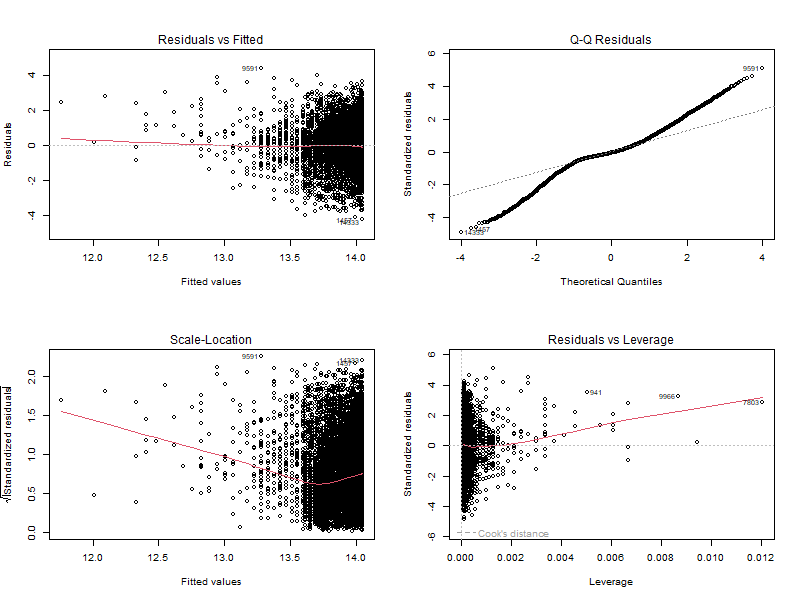
\includegraphics[width=\textwidth]{3.1 Salary vs Age.png}
    \label{fig:Residuales3}
    \scriptsize
    Source: Own calculation 
    \tiny
\end{figure}
The top right plot demonstrates clear non-normality of the residuals, with pronounced heavy tails. The top left plot reveals heteroscedasticity, as evidenced by the funnel shape, suggesting that residual variance increases with higher fitted values. The bottom left plot exhibits a skewed quadratic pattern, particularly between the 13.5 and 14.0 fitted value range, indicating lower residual variance in the middle range and higher variance at the extremes. Lastly, despite the removal of high-leverage points, the "Residuals vs Leverage" plot still shows a few influential points affecting the model. These observations suggest considering variance-stabilizing transformations or employing robust statistical methods to improve model performance.

\subsection{Peak age}

Given equation (1), we take the derivative with respect to \text{Age} and set it to zero:

\begin{equation}
\frac{d \log(w)}{d \text{Age}} = \beta_2 + 2 \beta_3 \text{Age} = 0 
\implies \text{Age} = -\frac{\beta_2}{2 \beta_3}
\end{equation}

At this point \text{Age} represents the "peak age" at which growth of earnings is maximized. Ensured given the concave shape of $\beta_3$. Figure \ref{fig:PEAKAGE} shows that peakage for monthly income salarial growth is reached at 41.77 years old, or between 41.12 and 42.45. 

\begin{figure}[H]
    \centering
    \caption{Peak age for labor income growth}
    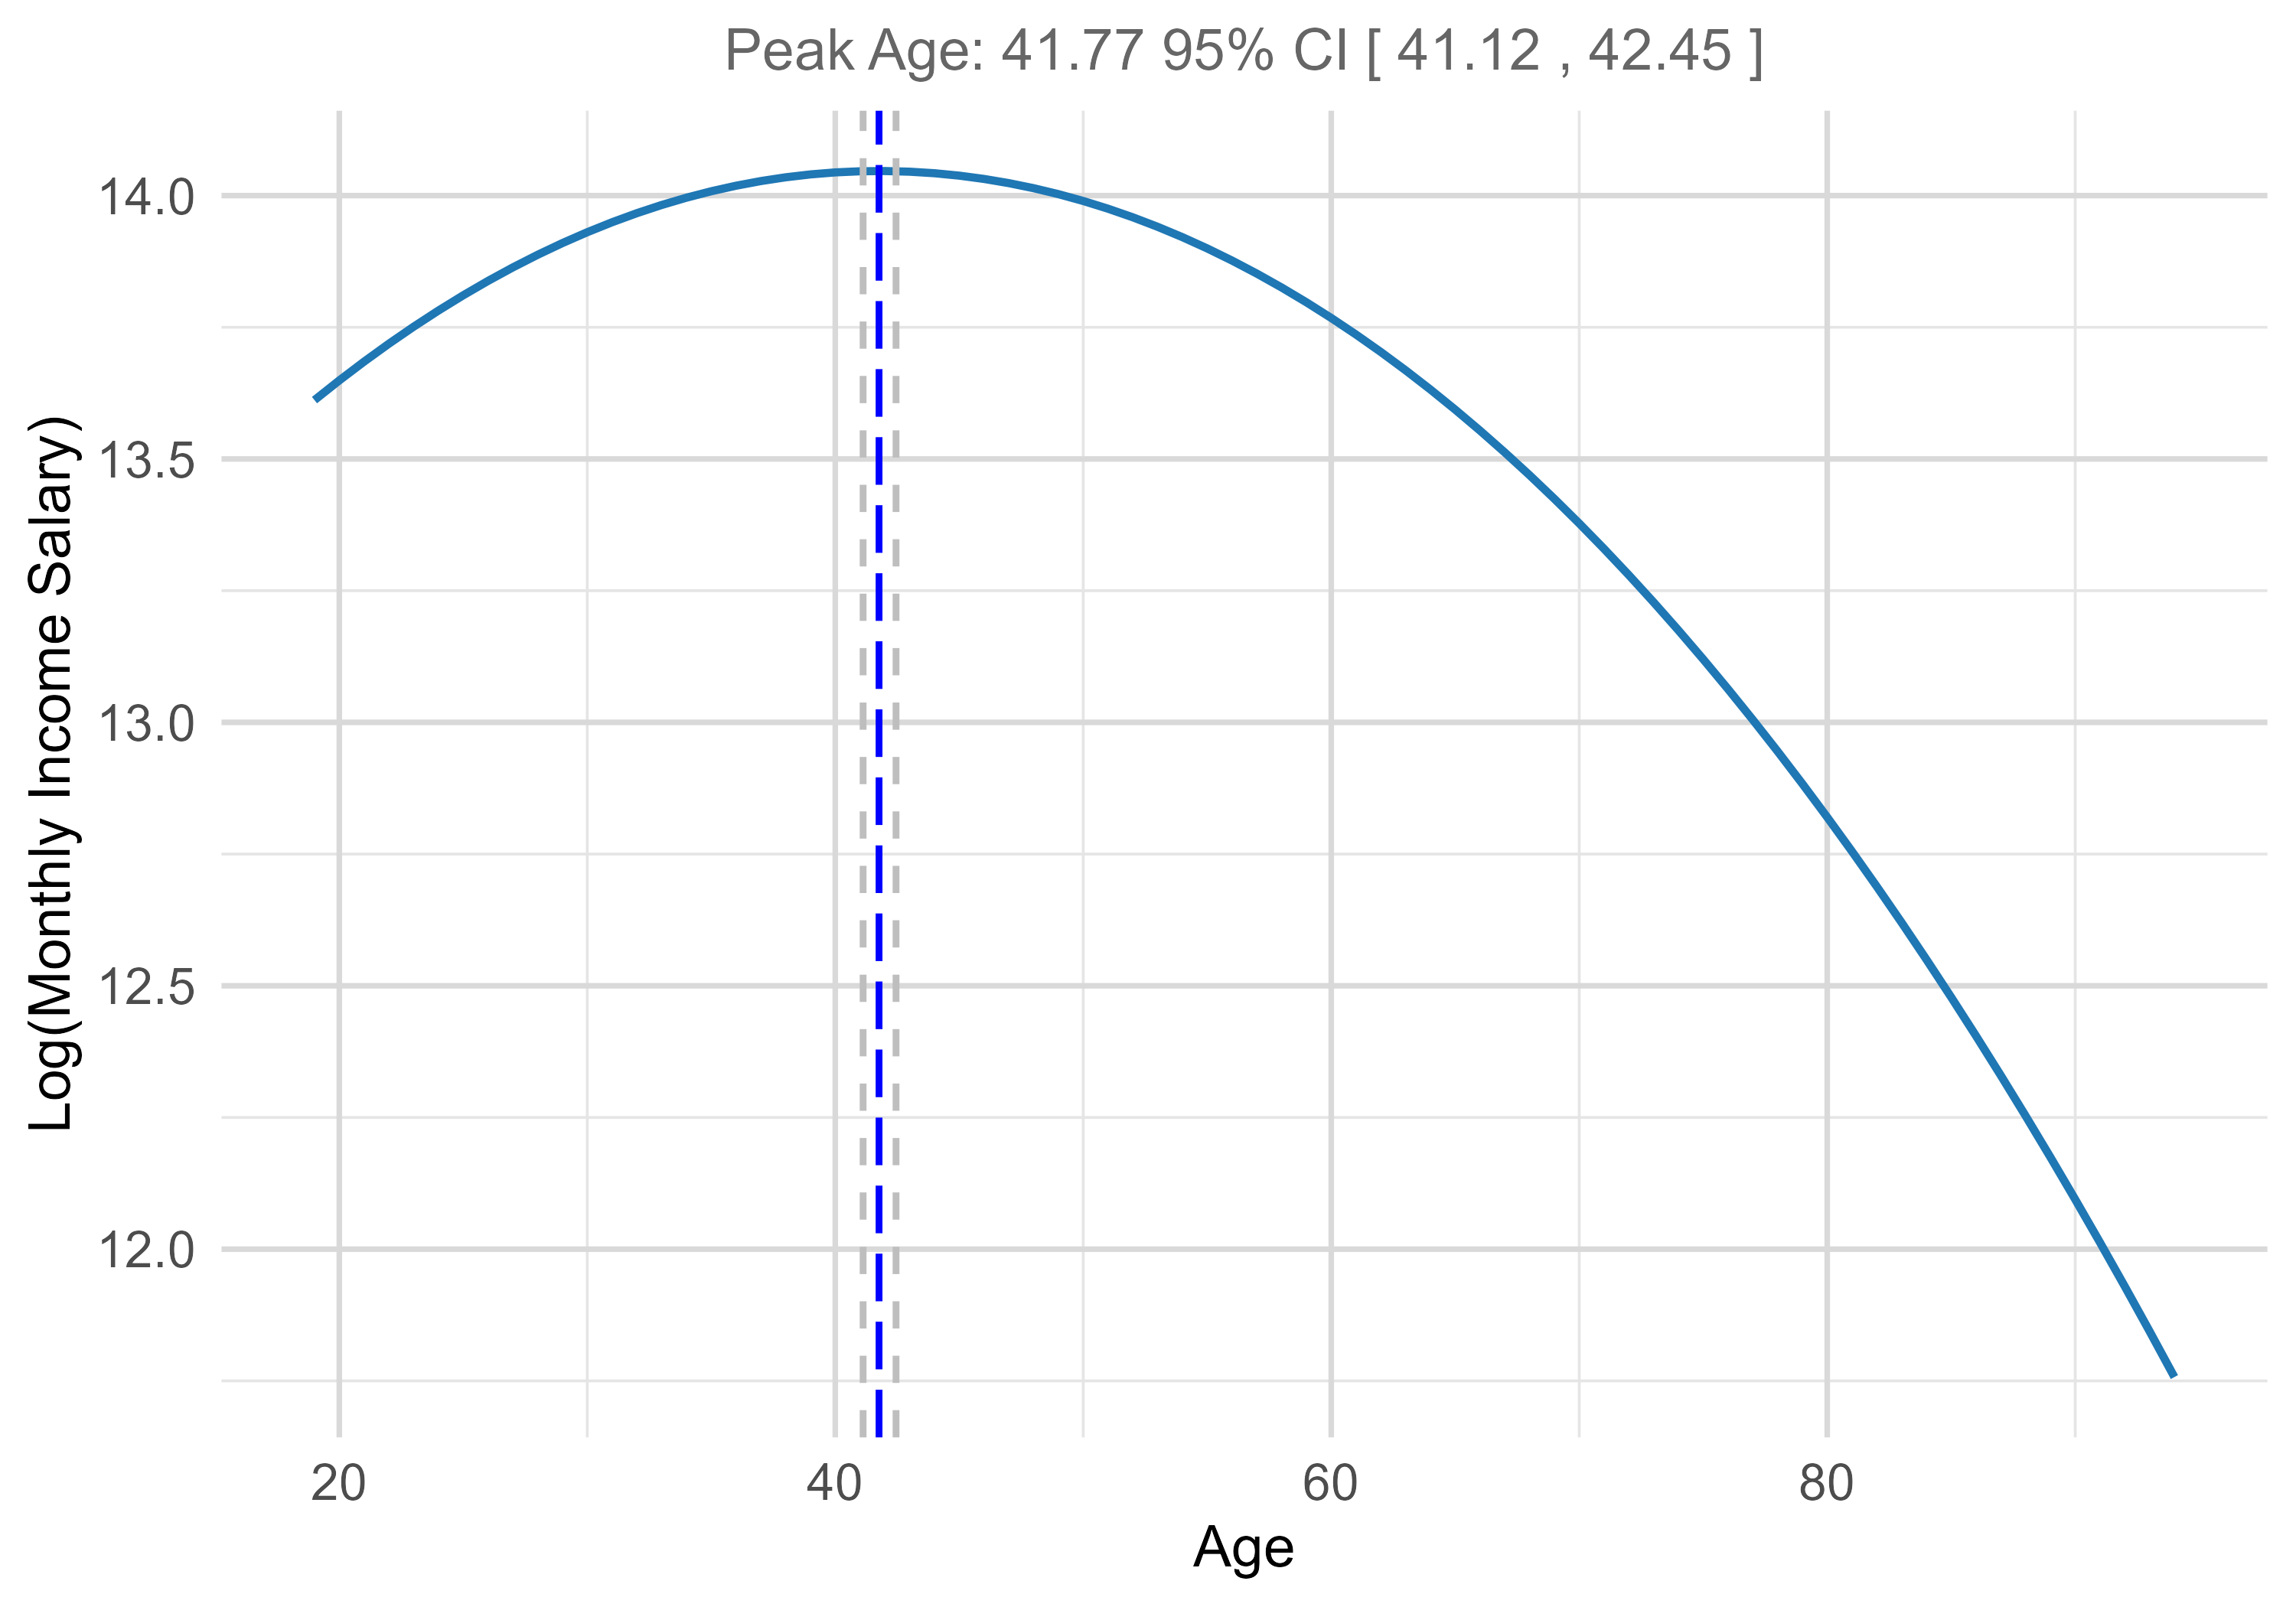
\includegraphics[width=\textwidth]{3.1PEAKAGE.png}
    \label{fig:PEAKAGE}
    \scriptsize % Smaller font size for the footnote
    \text{Source: Own calculation.Confidence intervals were calculated with bootstrap. Blue line corresponds to OLS peak age}
\end{figure}

In order to achieve this graphic, we constructed a function that took the coefficients from equation (1) and calculated equation (2). We used this function to generate confidence intervals with boostrap, with samples of 1000 observations, in order reduce uncertainty of the results. We then fitted equation (1) using the full dataset and generated predicted log-salaries for a range of ages between the minimun and the maximum age on the data base. The maxium is exactly achieved at log = 14.05 \( COP: 1'259.945\) at 41.77 years. Yet, as R and R adjusted measured indicate that the model fails to capture labor monthly income variance, we do not believe the peak age of this model is reliable as predictions. 

\section{Gender Earnings Gap}
The gender earnings gap has been a topic of significant concern among policymakers for decades, as it revolves around the persistent disparity in wages between male and female workers despite advances in gender equality. Understanding and addressing this gap is crucial for promoting fair and equitable labor markets. In this section, the gender wage gap is analyzed using three approaches. First, we estimate the unconditional wage gap. Second, we analyze the conditional wage gap using the Frisch-Waugh-Lovell (FWL) theorem, and third, we apply the FWL theorem with bootstrap to refine the conditional wage gap estimation. Finally, we plot the predicted age-wage profile to estimate the peak ages for each gender.

\subsection{ Unconditional and Conditional models}
We begin by estimating the unconditional wage gap:
\begin{equation}
    \log(w) = \beta_1 + \beta_2 \text{Female} + u
\end{equation}

Where Female is an indicator that takes 1 if the individual in the sample is
identified as female. 
The coefficient $\beta_2$ captures the percentage difference in wages between females and males, interpreted as the log-point difference in wages. A negative and statistically significant $\beta_2$ would indicate the presence of an unconditional gender wage gap.\\

To assess whether gender differences persist when accounting for observable worker and job characteristics we specified a conditional model that includes controls for age, education level, informality, and socioeconomic status (stratum) grounded in economic theory:
\begin{equation}
\log(w) = \beta_1+ \beta_2 \text{Female} + \beta_3 \text{Age} + \beta_4 \text{Age}^2 + \beta_5 \text{Education} + \beta_6 \text{Informal} + \beta_7 \text{Stratum} + \epsilon
\end{equation}


\begin{description}[leftmargin=0cm]
\item [Age and Age Squared:] Wages typically follow a concave age-earnings profile, reflecting human capital accumulation and depreciation over the life cycle (Mincer, 1974).

\item[Education:]  This variable contains the maximum educational level attained, and is a categorical ordinal variable, with categories ranging from 1 = None, 2 = Preschool, 3 = Primary incomplete, 4 = Primary complete, 5 = Secondary incomplete, 6 = Secondary complete, and 7 = Tertiary. We include this control based on the human capital theory (Becker, 1964), which suggests that higher levels of education increase productivity, leading to higher wages. Besides, Psacharopoulos (1985) provided empirical evidence supporting the effect of education on wages, that´s why it serves as a crucial control to isolate the gender wage gap from differences in skill levels.

\item[Informality:]  Informal is a dummy variable that equals 1 for individuals in the informal sector (without social security) and 0 otherwise.
According to La Porta and Shleifer (2014) informal jobs often lack benefits and stability, which may result in lower wages. We include this variable to controls for differences in job quality and formality status.

\item [Socioeconomic Status (Stratum):] Stratum is a categorical variable that serves as a proxy for socioeconomic background, which can influence access to education, job opportunities, and ultimately, wages (Pastore 1982)(Bourguignon et al., 2007).
\end{description}

We apply the FWL theorem to estimate the conditional wage gap by first regressing $\log(w)$ and Female on the control variables separately, and then regressing the residuals. This method provides the coefficient $\beta$ directly, demonstrating the partial effect of being female on wages while controlling for other factors. Theory says Female coefficient obtained through this method is numerically equivalent to the coefficient derived from the ordinary least squares (OLS) estimation of the full conditional model,to verify this, we also estimate the conditional model using OLS directly.

To assess the robustness of our estimates, we apply the bootstrap method to compute standard errors. The bootstrap involves repeatedly resampling the data with replacement and re-estimating the model, providing empirical distributions for our coefficients and their standard errors. Comparing the FWL and FWL with bootstrap results will highlight any discrepancies in inference due to sampling variability.


\subsection{Comparison between models}
The following Table~\ref{tab:gender_wage_gap} presents a comparison of four different approaches to estimating the gender wage gap.

\begin{table}[H]
\centering
\caption{Comparison of Unconditional and Conditional Gender Wage Gaps}
\label{tab:gender_wage_gap}
\resizebox{\textwidth}{!}{%
\begin{tabular}{@{\extracolsep{5pt}}lcccc}
\hline \hline \\[-1.8ex]
 & (1) & (2) & (3) & (4) \\
\hline \\[-1.8ex]
Female & $-0.229^{***}$ & $-0.301^{***}$ & $-0.301^{***}$ & $-0.301^{***}$ \\
 & (0.014) & (0.011) & (0.011) & (0.016) \\
\hline 
Method & Unconditional OLS & Conditional OLS & FWL & Bootstrap \\
Observations & 15,716 & 15,716 & 15,716 & 15,716 \\
R$^{2}$ & 0.017 & 0.436 & 0.048 & 0.506 \\
Adjusted R$^{2}$ & 0.017 & 0.436 & 0.048 & 0.506 \\
Residual Std. Error & 0.877 & 0.665 & 0.664 & 0.991 \\
Degrees of Freedom & 15,714 & 15,702 & 15,714 & 15,714 \\
F Statistic & 266.961$^{***}$ & 933.738$^{***}$ & 792.570$^{***}$ & 16,081.230$^{***}$ \\
\hline \hline \\[-1.8ex]
\multicolumn{5}{p{0.9\linewidth}}{\textit{Note:} $^{*}$p$<$0.1; $^{**}$p$<$0.05; $^{***}$p$<$0.01. Control variables for models 2, 3, and 4 include: age, maxEducLevel, informal, and estrato1.}
\end{tabular}
}%
\end{table}
The first model (Column 1) shows the unconditional gender wage gap without controlling for any other factors,and reveals a statistically significant gender effect with a coefficient of -0.229. However, the $R^2$ is very low at just 0.0167, indicating that the model explains only about 1.7\% of the variation in log incomes suggesting that gender alone is an insufficient predictor of income differences.

More problematically, the diagnostic tests shown in Table~\ref{tab:unconditional_model_results} reveal violations of key OLS assumptions. The Breusch-Pagan test shows a highly significant result (\textit{p}-value $<$ 2.2e-16), providing strong evidence of heteroskedasticity. Additionally, the Durbin-Watson test indicates significant autocorrelation (DW = 1.6388, \textit{p}-value $<$ 2.2e-16). These violations suggest that standard errors from the conventional OLS approach are likely unreliable, therefore, robust standard errors were used to account for these issues and ensure statistical inference.


\begin{table}[H]
\caption{Unconditional Model Results} 
\label{tab:unconditional_model_results}
\centering
\vspace{0.5cm} % Ajusta el espacio aquí
\begin{tabular}{lcc}
    \textbf{Description} & \textbf{Value} \\ 
    \hline \hline
    Mean of residuals & -0.00 \\ 
    P-value of Breusch-Pagan test & 2.2e-16\\ 
    P-value of Durbin-Watson test & 2.2e-16 \\ 
    \hline
\end{tabular}
\end{table}



Moving to Columns 2, 3, and 4, we see the results after controlling for factors such as age, education level, informal employment status, and socioeconomic stratum, and all three controlled models: Conditional OLS, Frisch-Waugh-Lovell (FWL), and FWL with Bootstrap, show a larger gender wage gap of 30.1\% .

The in-sample fit reveal important differences in explanatory power. The R² values indicate that while the unconditional model explains only 1.7\% of wage variation, the Conditional OLS and Bootstrap models explain approximately 43.6\% and 50.6\% respectively, and the FWL model a 4.8\%, which is expected given  on isolating the effect of gender. 

With the coefficient of models 2 and 3 we confirm that the FWL estimator is numerically identical to the OLS estimator, validating the theoretical equivalence between the two methods. 

In the FWL model, the standard error for the female coefficient is 0.011 and it´s calculated based on the classical assumptions of the linear regression model, however, the diagnostic tests (see table ~\ref{tab:fwl_model_results}) reveal violations of these assumptions. Although the VIF analysis indicates multicollinearity between age and age-squared, this is expected and not problematic since age-squared is included to capture non-linear effects; the Breusch-Pagan test shows significant heteroskedasticity, and the Durbin-Watson test indicates the presence of autocorrelation . These violations suggest that the  standard error calculation may not accurately reflect the true uncertainty in the coefficient estimate. In contrast, the bootstrap approach yields a larger standard error of 0.016 for the same coefficient, with a 45\% increase in the standard error that reflects the additional uncertainty captured by the bootstrap method, as it repeatedly resamples the data to generate an empirical distribution of coefficient estimates and this process naturally incorporates the heteroskedasticity and autocorrelation present in your data.

\begin{table}[H]
\caption{FWL Model Results} 
\label{tab:fwl_model_results}
\centering
\vspace{0.5cm} % Ajusta el espacio aquí
\begin{tabular}{lcc}
    \textbf{Description} & \textbf{Value} \\ 
    \hline \hline
    Mean of residuals & -0.00 \\ 
    P-value of Breusch-Pagan test & 1.380e-12 \\ 
    P-value of Durbin-Watson test & 1.662e-11 \\ 
    \hline
\end{tabular}
\end{table}

After correcting for robust standard errors and improving statistical significance, we can interpret the coefficients associated with gender. The 30.1\% gap, which persists after accounting for productivity-related factors, suggests discrimination rather than just a selection problem, if the gap had decreased substantially after adding controls, it would have indicated that differences in characteristics explain much of the wage differential. Instead, the widening gap points to some possible explanations: direct wage discrimination where women are paid less for equal work; occupational segregation where women are concentrated in lower-paying occupations despite similar qualifications; or unobserved factors not captured in the model, such as work hours flexibility preferences or career interruptions.


\subsection{ Peak ages}

We also study gender age-wage patterns by estimating separate earnings models for men and women. To identify peak earning ages, we derivative the wage function, then we applied the delta method to construct confidence intervals around these peak age estimates, accounting for coefficient uncertainty.
The analysis also involved creating visualizations of the age-wage profiles, which required generating predictions across the age spectrum and properly back-transforming the log-wages to monetary values using the exponential function. \\

The figure \ref{fig:Predicted age-wage profile by gender} reveals gender-specific earning trajectories, with indicators marking the estimated peak ages and confidence bands illustrating prediction uncertainty. This approach allows us for direct comparison of peak earning ages between genders while controlling for important socioeconomic factors.

\begin{figure}[H]
    \centering
    \caption{Predicted age-wage profile by gender}
    \label{fig:Predicted age-wage profile by gender}
    \includegraphics[width=0.7\textwidth]{age_wage_profile.png}
\end{figure}

Examining this wage trajectory, we find critical insights into the gender wage gap that go beyond simple aggregate comparisons. The differentiated timing of peak earnings with non-overlapping confidence intervals represents a temporal dimension of gender wage inequality that standard cross-sectional analyses often miss. The data suggests the wage gap isn't merely about absolute values, it's structurally embedded in  trajectories themselves. Women reach their maximum earning potential approximately 5.64 years earlier than men, so this pattern likely reflects the cumulative effect of systemic factors including differential promotion rates, career interruptions, occupational segregation, and possibly discriminatory evaluation practices. The steeper post-peak decline for women further compounds lifetime earning disparities, these age-dependent patterns indicate that any comprehensive model of the gender wage gap must account for the interaction between age and gender—not as separate features, but as deeply intertwined variables that together shape earnings throughout the career lifecycle. This temporal asymmetry in wage trajectories represents a manifestation of gender inequality.

\begin{table}[!htbp] \centering
  \caption{Summary of Peak Age and Wage by Gender}
  \label{tab:peak_age_wage}
\begin{tabular}{@{\extracolsep{5pt}} lcccc}
\hline
Gender & Peak Age & Lower CI Limit & Upper CI Limit & Peak Wage \\
\hline
Female & $40.27$ & $39.29$ & $41.26$ & $1,173,676.00$ \\
Male & $45.91$ & $45.12$ & $46.71$ & $1,473,778.00$ \\
\hline
\end{tabular}
\end{table}

\section{Predicting Earnings}

In order to evaluate the predictive power of the previous specifications and five additional models we performed the Validation Set (VS) and Leave One Out Cross-Validation (LOOCV) approaches to assess the fit in test samples. The equations that describe the models that were fitted:
\begin{flalign}
    \log(w) &= \beta_0 + \beta_1 \text{Age} + \beta_2 \text{Age}^2 + u \tag{1} \\  
    \log(w) &= \beta_0 + \beta_1 \text{Female} + u \tag{2} \\  
    \log(w) &= \beta_0 + \beta_1 \text{Female} + \beta_2 \text{Age} + \beta_3 \text{Age}^2 \notag \\  
    &\quad + \beta_4 \text{Education} + \beta_5 \text{Informal} + \beta_6 \text{Stratum} + u \tag{3} \\  
    \log(w) &= \beta_0 + \beta_1 \text{Female} + \beta_2 \text{Age} + \beta_3 \text{Age}^2 \notag \\  
    &\quad + \beta_4 \text{Education} + \beta_5 \text{Informal} + \beta_6 \text{Stratum} + \beta_7 \text{Occupation} + u \tag{4} \\  
    \log(w) &= \beta_0 + \beta_1 \text{Female} + \beta_2 \text{Education} + \beta_3 (\text{Female} \times \text{Education}) \notag \\  
    &\quad + \beta_4 \text{Age} + \beta_5 \text{Age}^2 + \beta_6 \text{Informal} + \beta_7 \text{Stratum} + \beta_8 \text{Occupation} + u \tag{5} \\  
    \log(w) &= \beta_0 + \beta_1 \text{Female} + \beta_2 \text{Education} + \beta_3 (\text{Female} \times \text{Education}) \notag \\  
    &\quad + \beta_4 \text{Age} + \beta_5 \text{Age}^2 + \beta_6 \text{Age}^3 + \beta_7 \text{Informal} + \beta_8 \text{Education} \notag \\  
    &\quad + \beta_9 (\text{Informal} \times \text{Education}) + \beta_{10} \text{Stratum} + \beta_{11} \text{Occupation} + u \tag{6} \\  
    \log(w) &= \beta_0 + \beta_1 \text{Female} + \beta_2 \text{Education} + \beta_3 (\text{Female} \times \text{Education}) \notag \\  
    &\quad + \beta_4 \text{Age} + \beta_5 \text{Age}^2 + \beta_6 \text{Age}^3 + \beta_6 \text{Informal} + \beta_7 \text{Education} \notag \\  
    &\quad + \beta_8 (\text{Informal} \times \text{Education}) + \beta_9 \text{Stratum} + \beta_{10} \text{Education} \notag \\  
    &\quad + \beta_{11} (\text{Stratum} \times \text{Education}) + \beta_{12} \text{Occupation} + u \tag{7} \\  
    \log(w) &= \beta_0 + \beta_1 \text{Female} + \beta_2 \text{Education} + \beta_3 \text{Stratum} + \beta_4 (\text{Female} \times \text{Education} \times \text{Stratum}) \notag \\  
    &\quad + \beta_5 \text{Age} + \beta_6 \text{Age}^2 + \beta_7 \text{Age}^3 + \beta_8 \text{Informal} + \beta_9 \text{Education} \notag \\  
    &\quad + \beta_{10} (\text{Informal} \times \text{Education})  + \beta_{12} \text{Occupation} + u \tag{8}  
\end{flalign}

The  Table \ref{tab:accuracy} shows the predictive performance of the previous specifications in the test sample with the VS approach, that allows us to assess the predictive performance of models by comparing their errors on an testing dataset:

The following Table shows the predictive performance of the previous specifications in the test sample with the VS approach, that allows us to assess the predictive performance of models by comparing their errors on an testing dataset:

\begin{table}[H] 
    \centering 
    \caption{Predictive performance of each model} 
    \label{tab:accuracy} 
    \resizebox{\textwidth}{!}{ % Ajusta la tabla al ancho de la página
    \begin{tabular}{@{\extracolsep{5pt}} cccccccccc} 
    \hline \hline \\[-1.8ex] 
     & & \multicolumn{8}{c}{\textbf{Model}} \\ 
     \cline{3-10} \\[-1.8ex]  
     & \textbf{Metric} & \textbf{(1)} & \textbf{(2)} & \textbf{(3)} & \textbf{(4)} & \textbf{(5)} & \textbf{(6)} & \textbf{(7)} & \textbf{(8)}  \\ 
    \hline \\[-1.8ex] 
     & RMSE & 2338267 &2347259 &1857504& 1809635& 1810657& 1804957& 1789173& 1787151 \\ 
     & MAE & 968001 & 970705& 768276& 753428& 750558& 748148& 744882& 745172 \\ 
     & MAPE & 92.623 & 93.962 &67.417& 65.691& 65.371& 65.641& 65.532 &65.394 \\
     & $R^2$ & 0.040 & 0.020 & 0.439 &0.460& 0.464& 0.465& 0.467 & 0.468 \\ 
    \hline \\[-1.8ex] 
    \multicolumn{10}{l}{Source: Own calculation.} 
    \end{tabular} 
    } % Cierre de resizebox
\end{table}

 In our case, the results above show a progressive improvement as more as more predictors and interaction terms are included, we observe an improvement in predictive accuracy, with lower RMSE and MAE values and an increasing $R^2$, reaching \$1'787.151 RMSE in the last model. However, a notable aspect of the results is the substantial gap between RMSE and MAE across all models. This suggests that the models may be struggling with certain extreme errors, likely due to the presence of outliers or high variance in some segments of the data. Since RMSE penalizes larger errors more heavily than MAE, this discrepancy highlights the potential impact of extreme deviations on model performance. In order to adress this issue, figures \ref{fig:Distribution of residuals} to \ref{fig:outliers} show a a careful residual analysis of the model $(8)$ to enhance predictive accuracy and identify the influence of extreme values on overall performance.  
 
 
\begin{figure}[H]
    \centering
    \caption{Distribution of residuals}
    \label{fig:Distribution of residuals}
    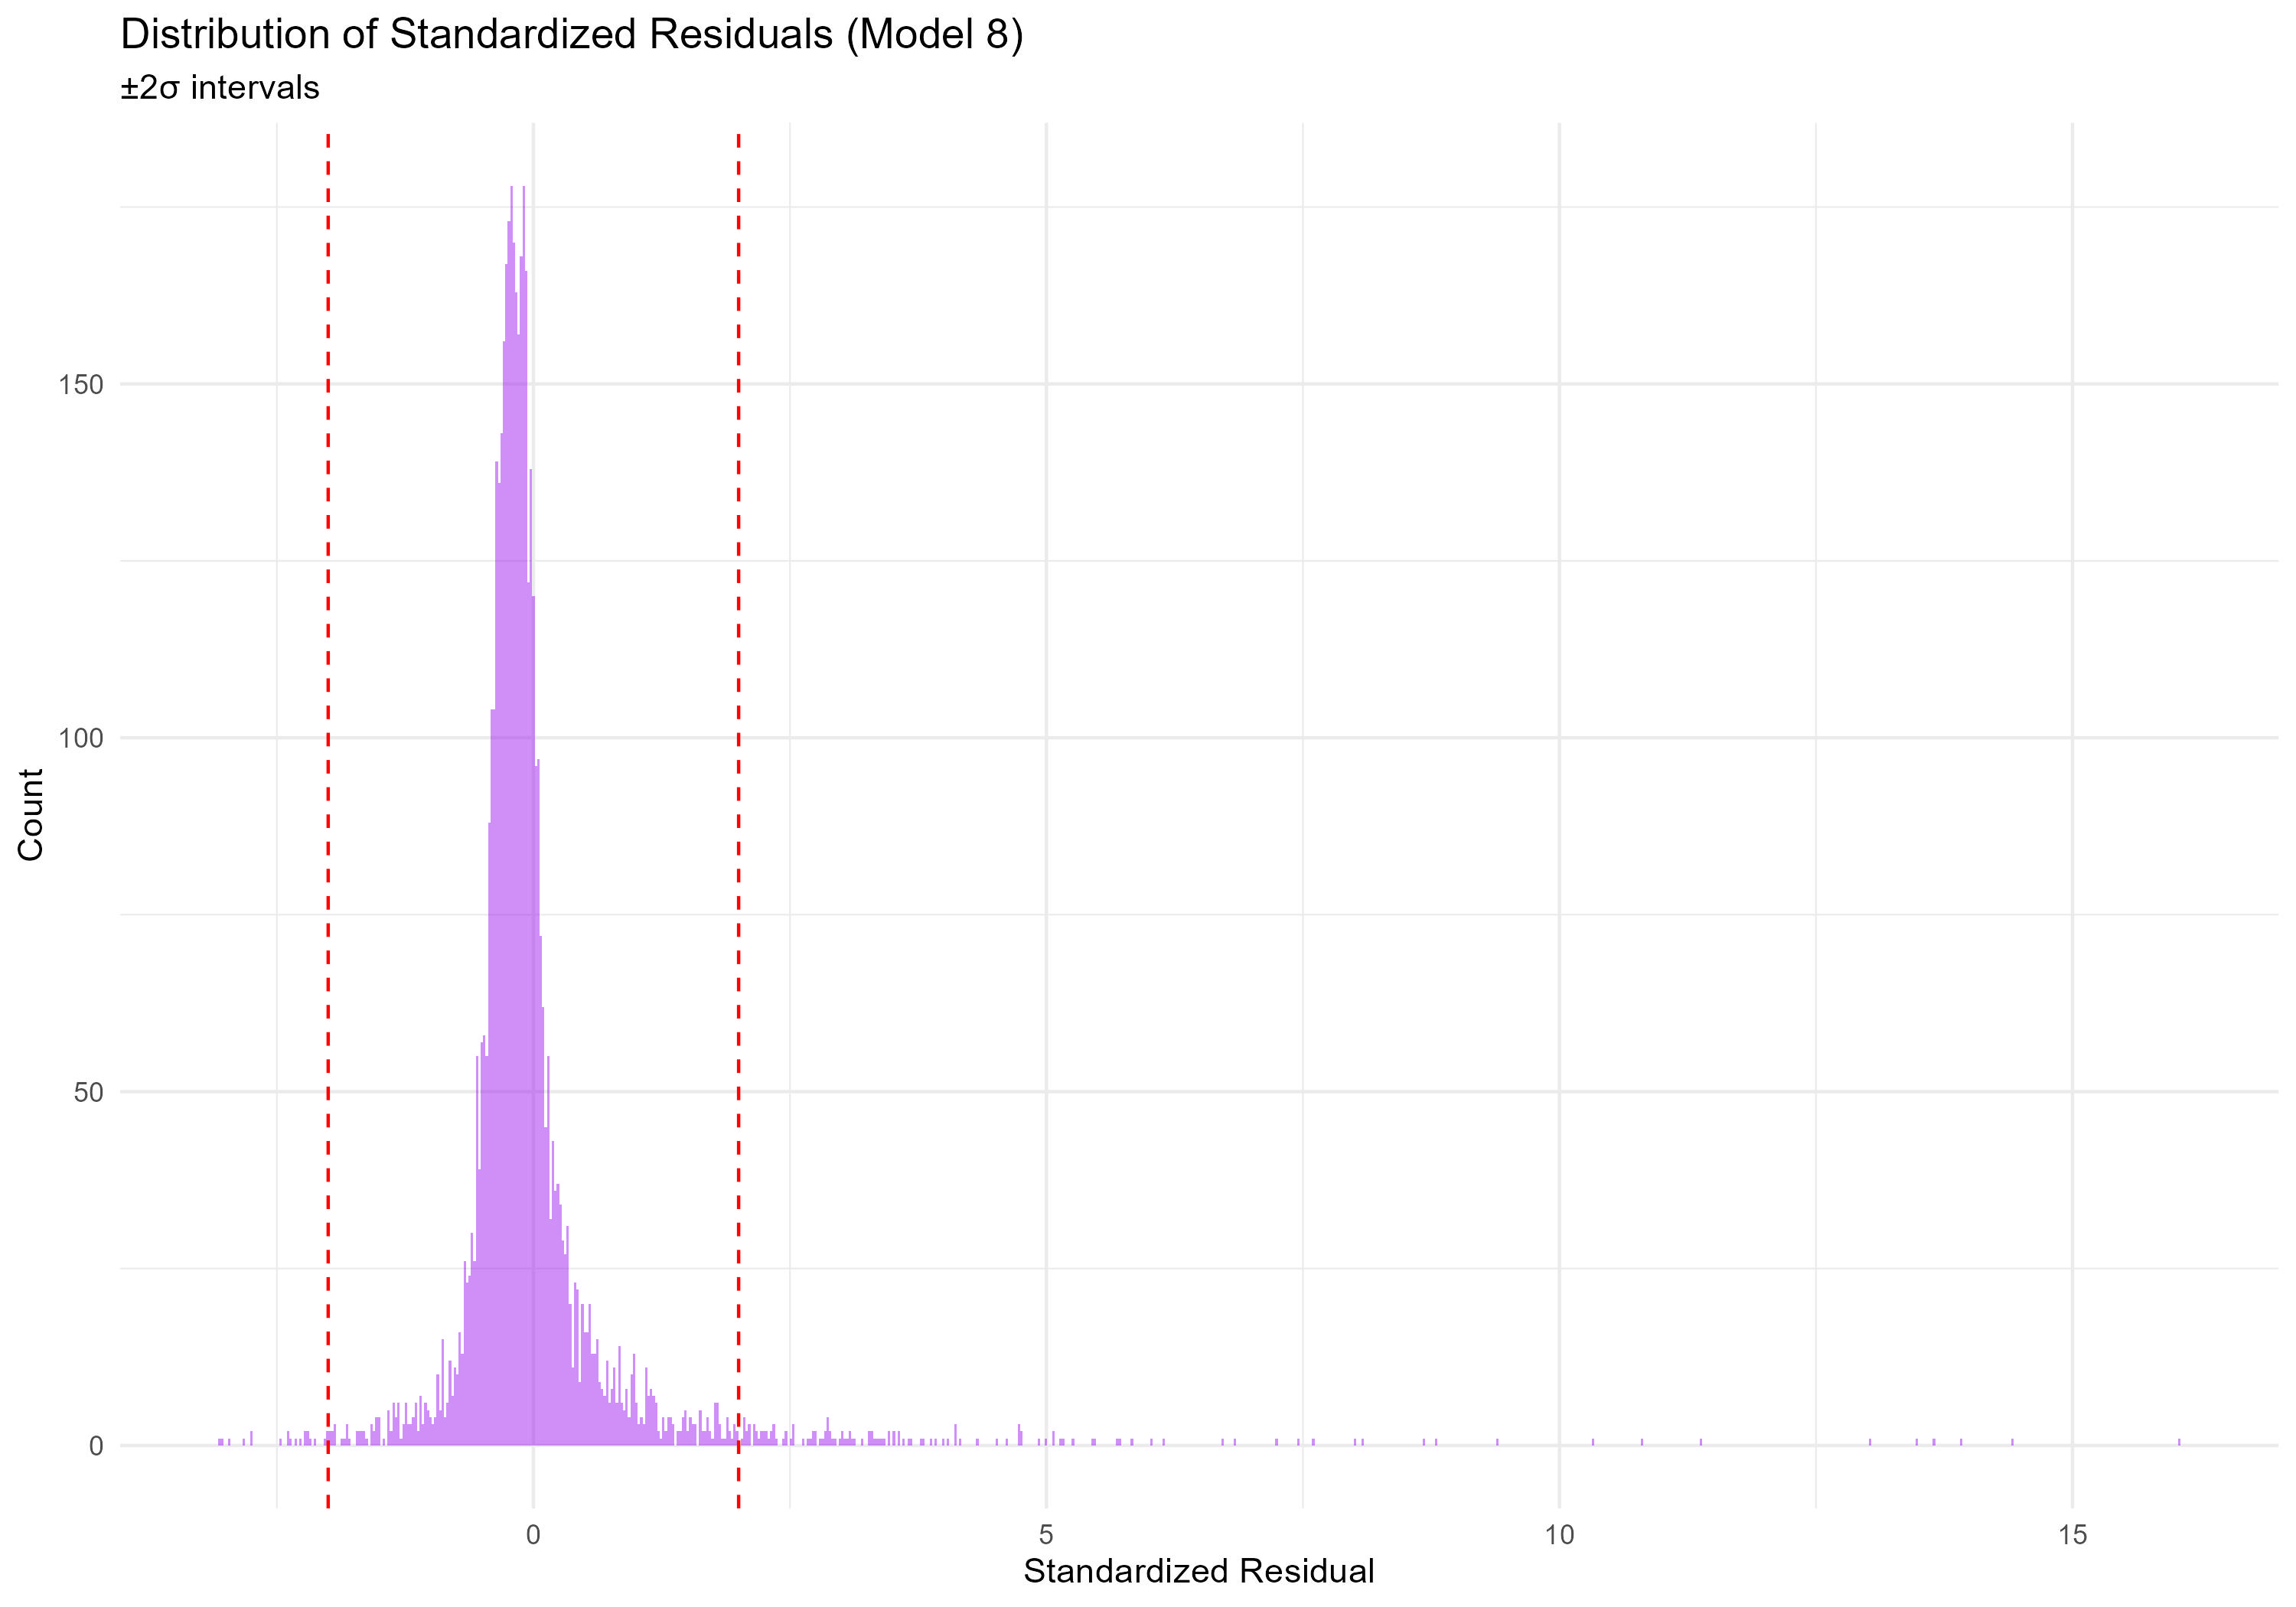
\includegraphics[width=0.8\textwidth,  height=0.5\textwidth]{Distribution_residuals.jpg}
\end{figure}

\begin{figure}[H]
    \centering
    \caption{Outliers in model (8)}
    \label{fig:residuals vs fitted}
    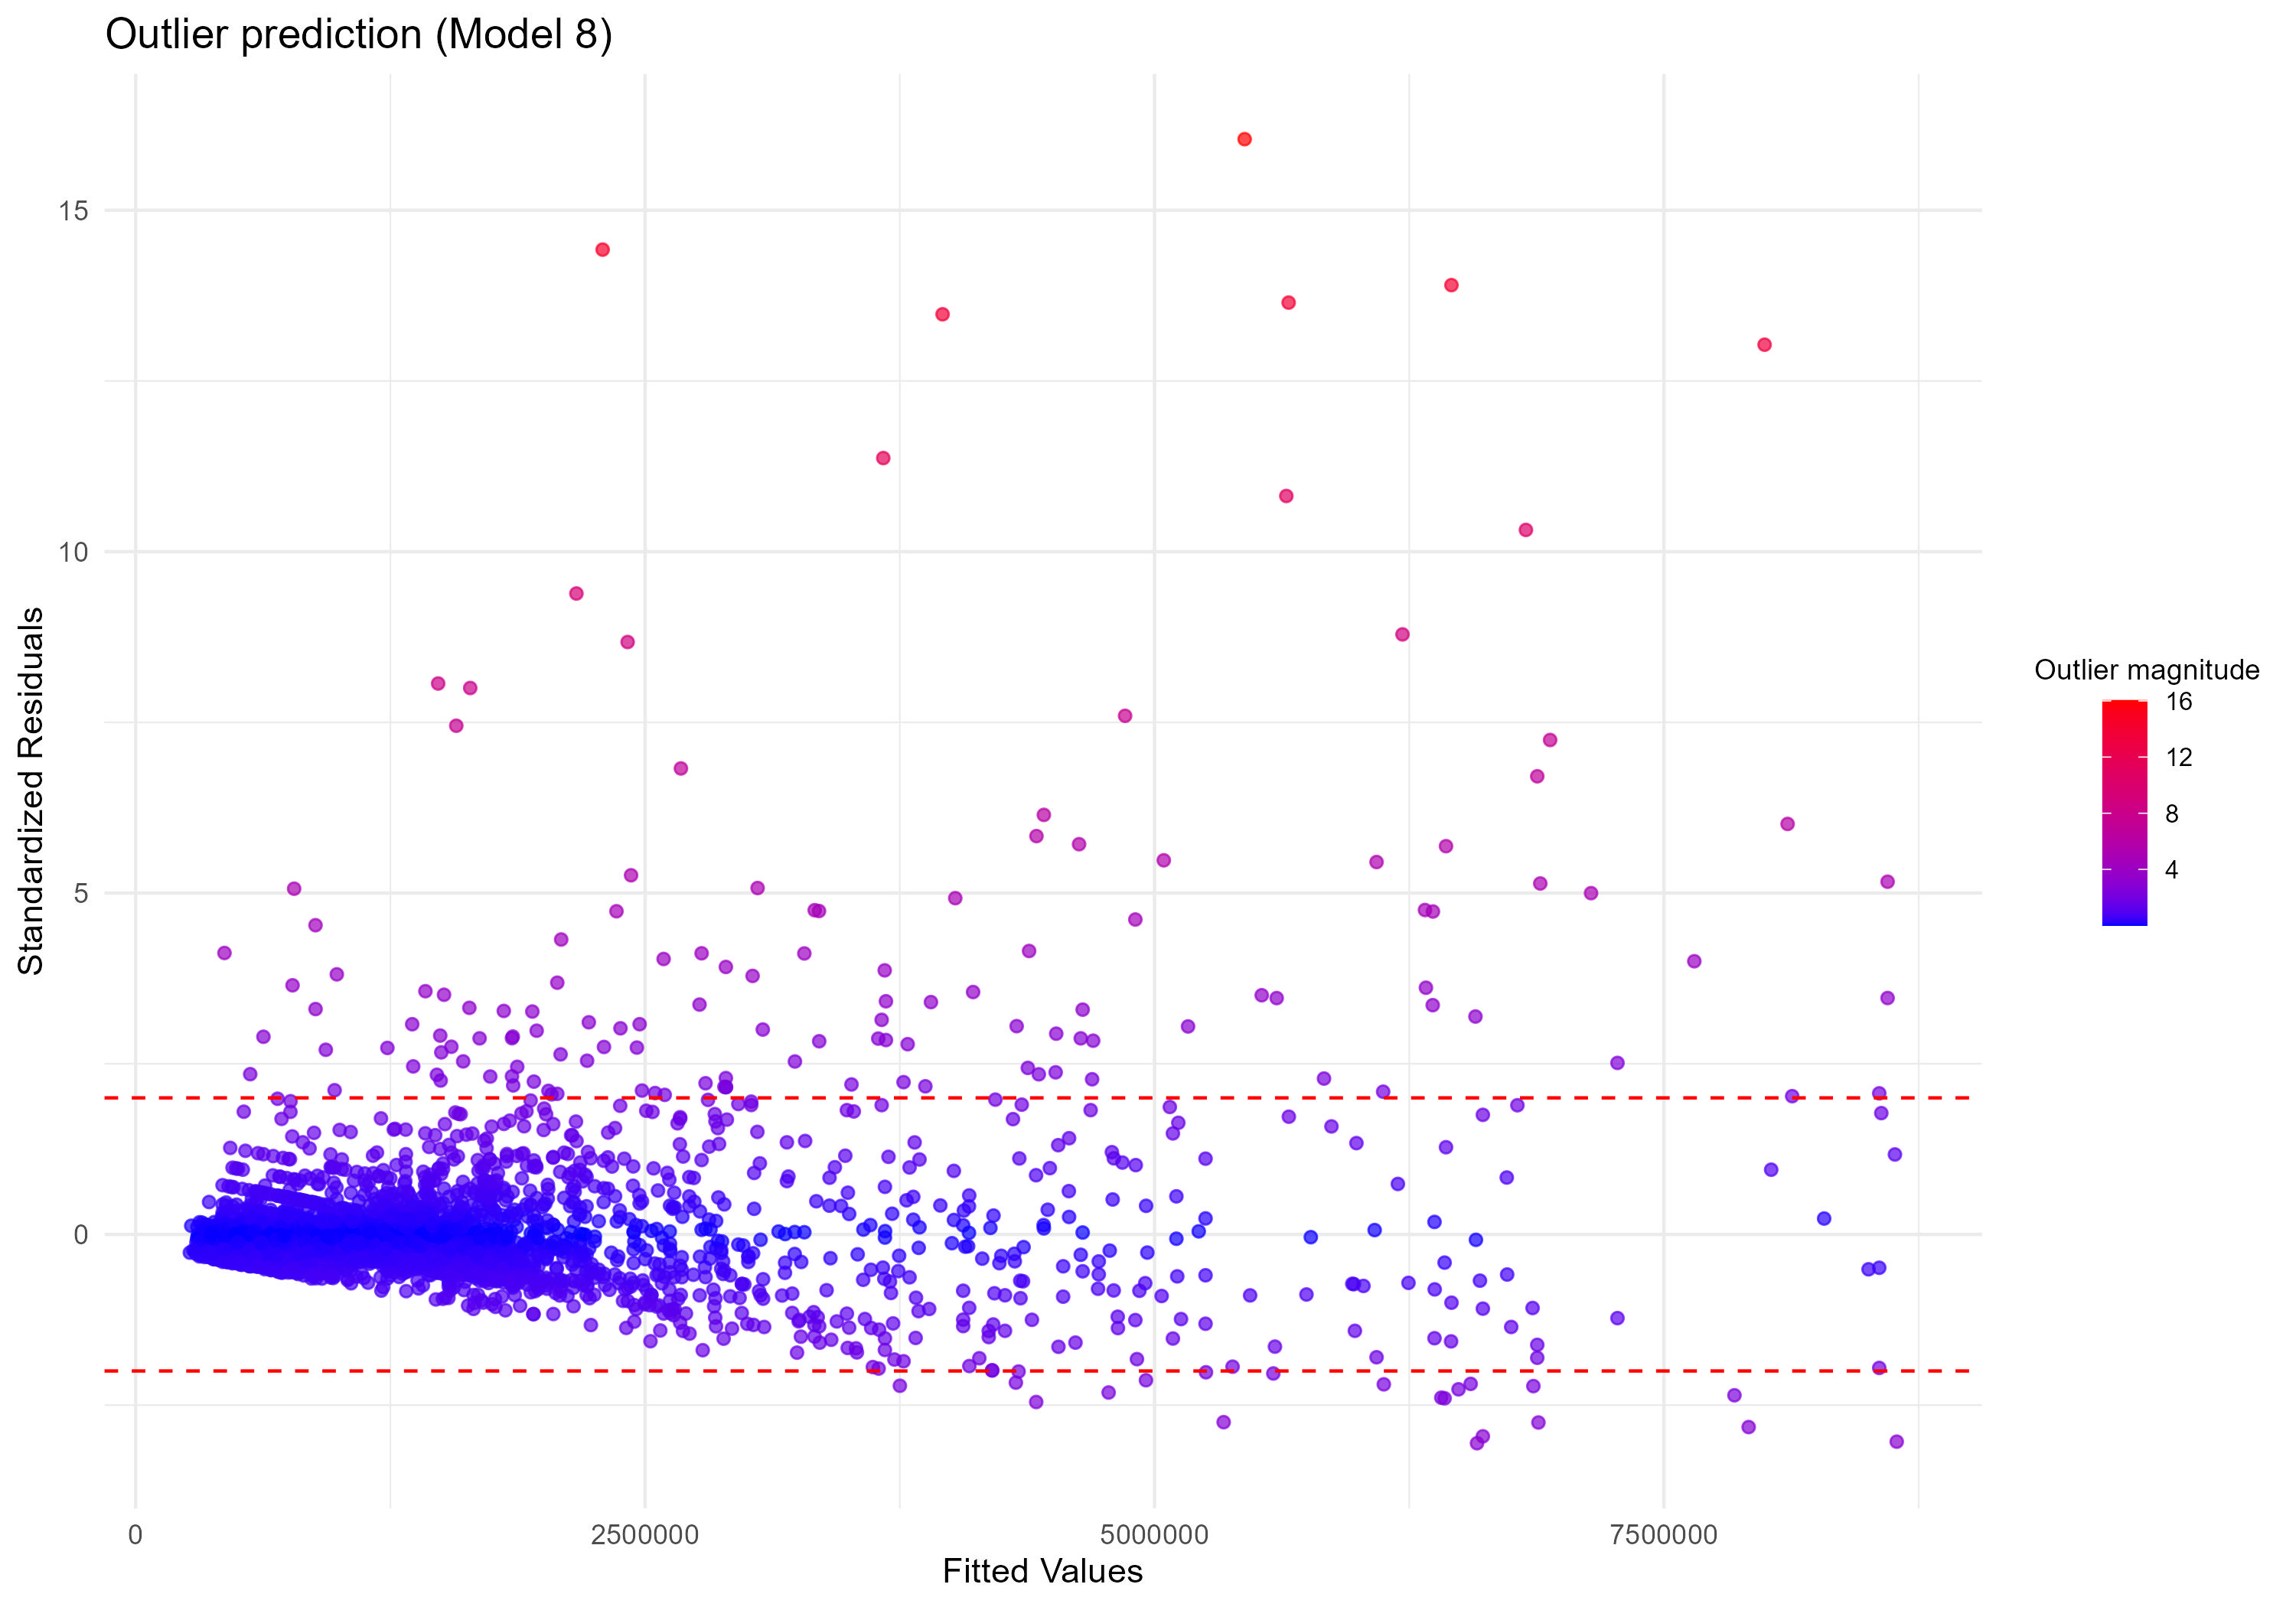
\includegraphics[width=0.8\textwidth]{resid_vs_fitted.jpg}
\end{figure}
\begin{figure}[H]
    \centering
    \caption{Outliers by occupation in model (8)}
    \label{fig:outliers}
    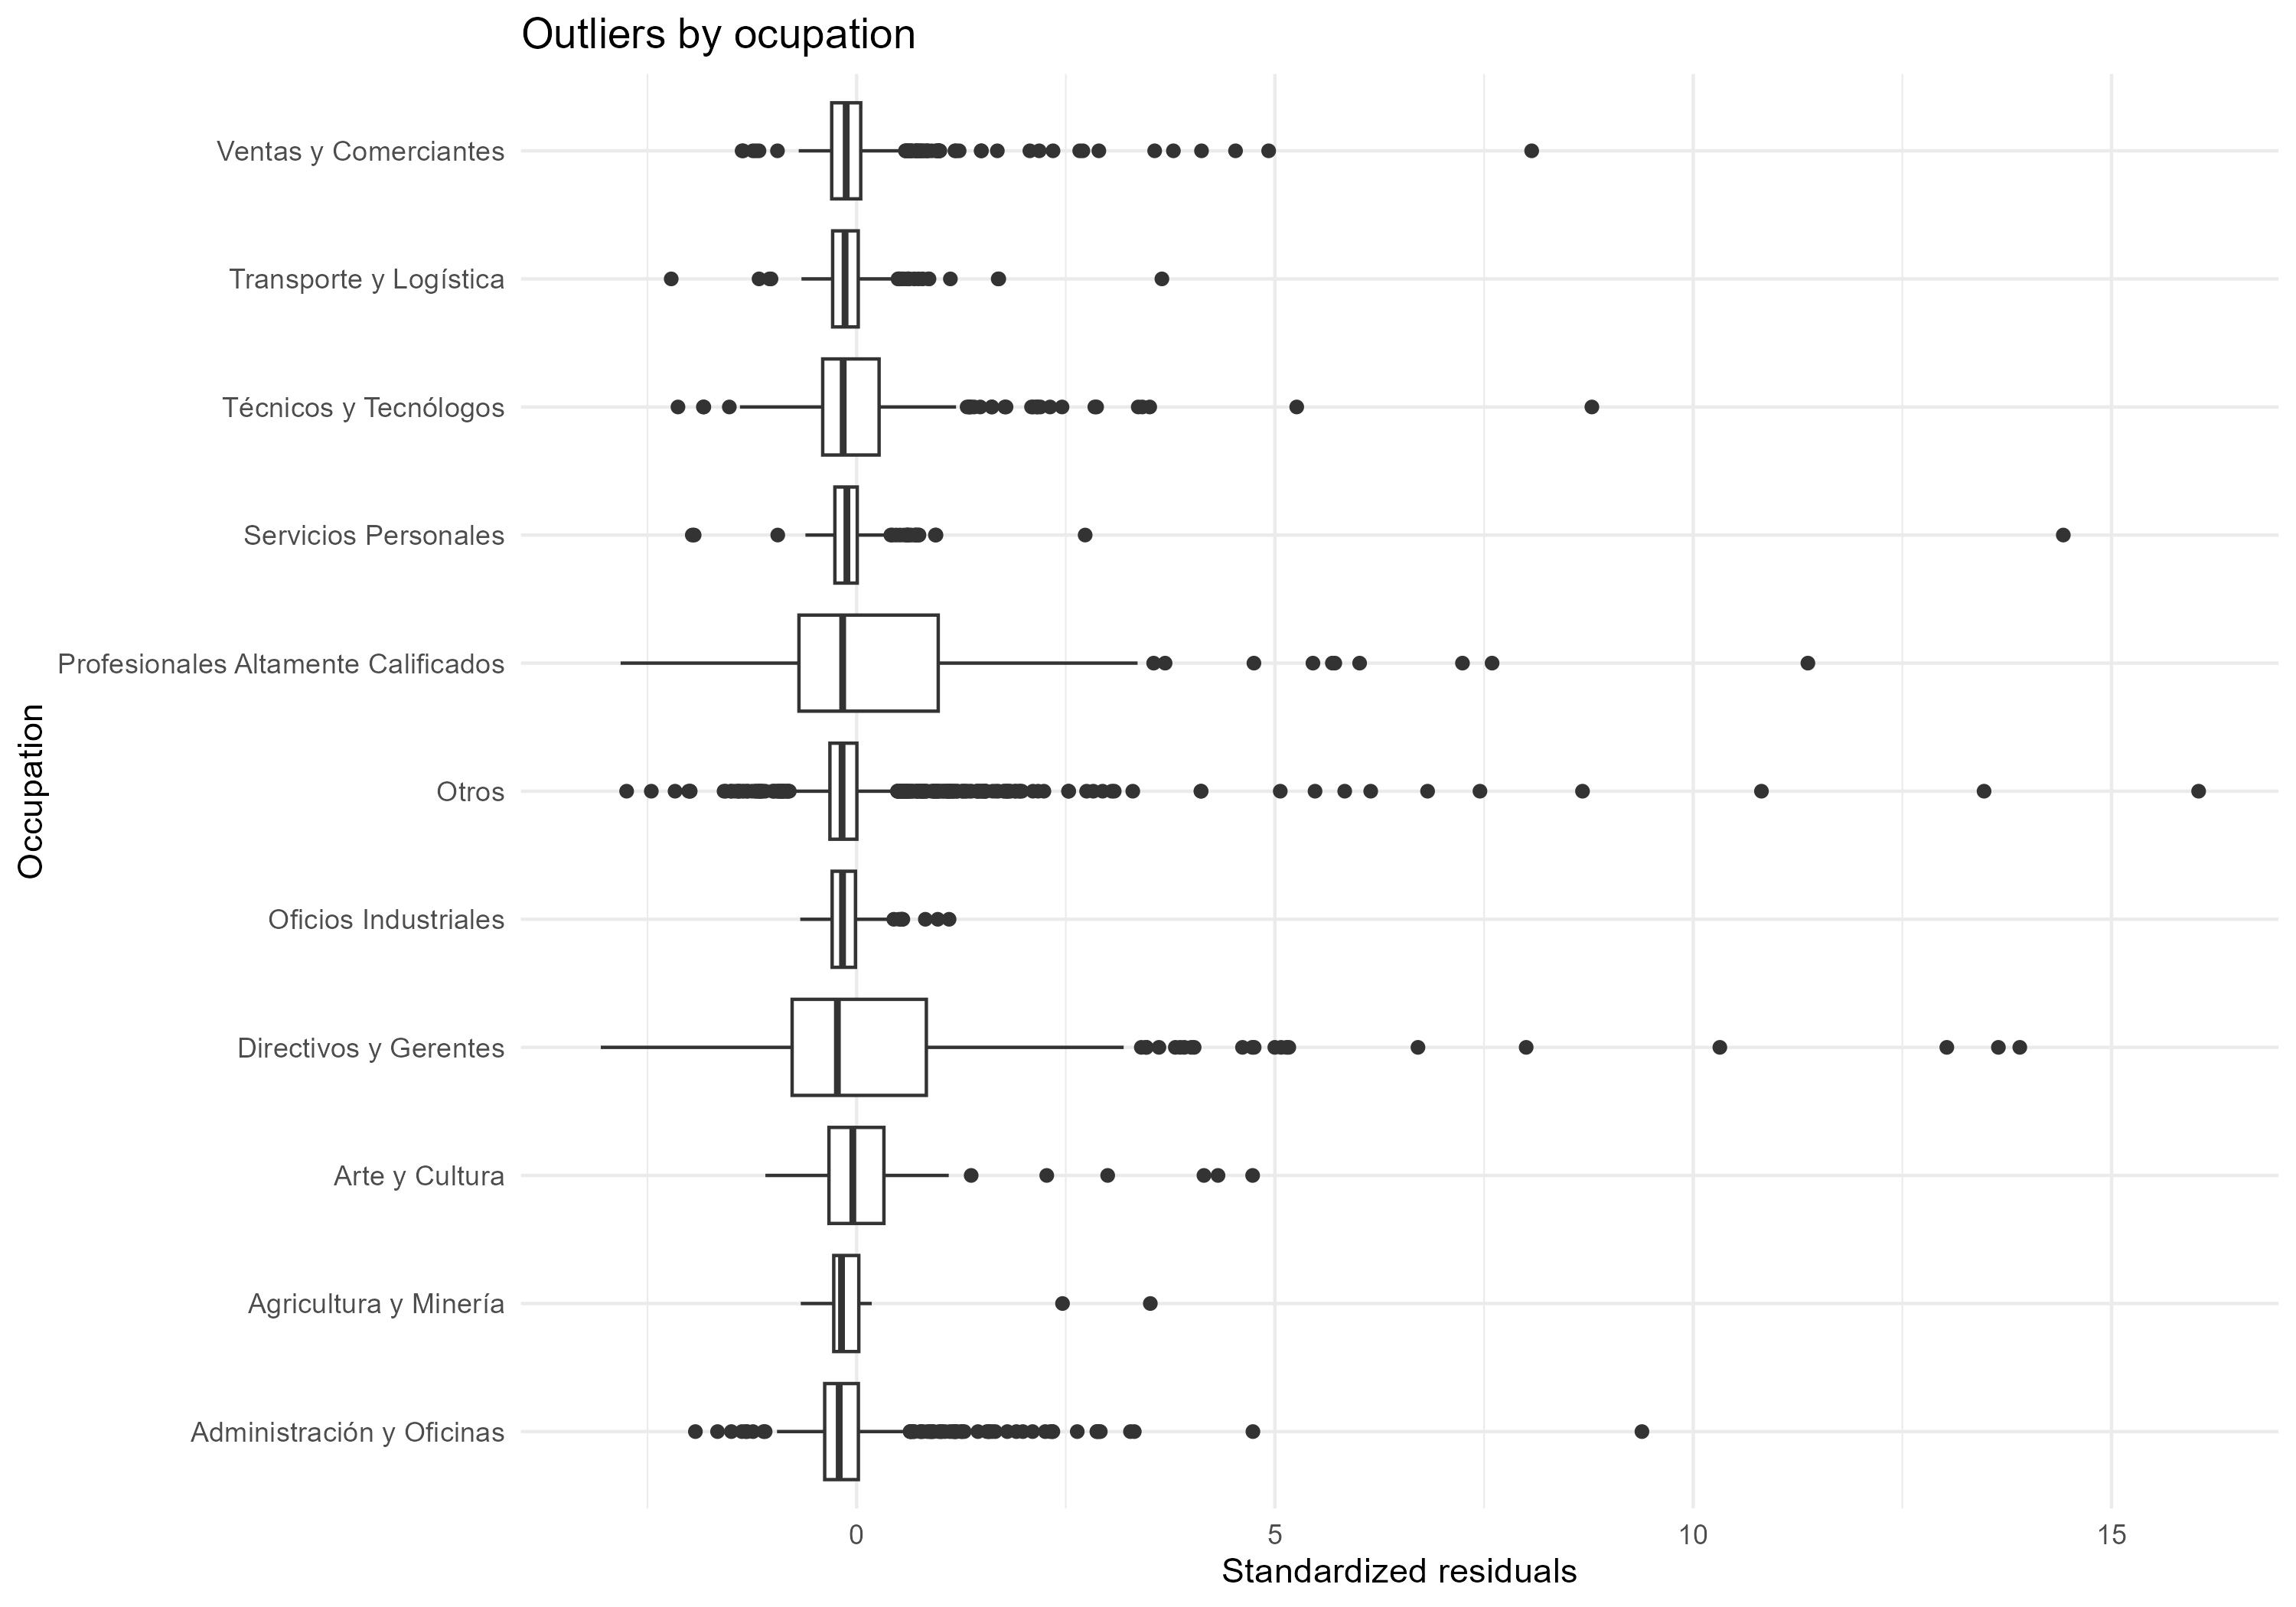
\includegraphics[width=0.8\textwidth]{out_by_ocup.jpg}
\end{figure}
Upon examining the most extreme cases, we notice that these outliers belong to high-income individuals (e.g., above 25,000,000 in total income), many of whom are in managerial or high-skill professional occupations (Directivos y Gerentes, Profesionales Altamente Calificados). These individuals tend to have the highest levels of education and reside in the wealthiest socioeconomic strata. The model systematically underpredicts their income, as indicated by their large positive residuals. This suggests potential issues with model specification—perhaps nonlinearities or interactions are not fully captured—or that important explanatory variables (such as firm ownership, additional sources of income, or network effects) are missing.

However, another noteworthy observation is that some individuals report an income significantly higher than what their observable characteristics would suggest (for example, an individual with income higher than \$28000000 but report to be fireman calls our atention). This raises questions about potential unreported factors influencing their earnings, and in some cases, could be a red flag for inconsistencies in income declaration. Given the magnitude of some residuals, tax authorities like DIAN may want to investigate whether all income sources are being properly declared.

\begin{table}[!htbp] 
    \centering 
    \small % Reduce el tamaño de la fuente de la tabla
    \caption{Results by Validation Approach} 
    \label{tab:LOOCV} 
    \begin{tabular}{@{\extracolsep{5pt}} ccccc} 
    \hline \hline \\[-1.8ex] 
    \multirow{2}{*}{\textbf{Method}} & \multicolumn{2}{c}{\textbf{Validation Set}} & \multicolumn{2}{c}{\textbf{LOOCV}} \\  
    \cline{2-5} \\[-1.8ex]  
     & \textbf{-} & \textbf{-} & \textbf{Furrr} & \textbf{Model D} \\ 
    \hline \\[-1.8ex] 
    Furr   & 1789173 & 1787151 & 2338267 & 752138.2 \\ 
    doParallel &  & 745172  &  & 1787151  \\ 
    \hline \\[-1.8ex] 
    \multicolumn{5}{l}{Source: Own calculation.} 
    \end{tabular} 
\end{table}

In Table \ref{tab:LOOCV}  we evaluate model performance using Leave-One-Out Cross-Validation (LOOCV), to do so we implemented two different approaches: one leveraging the package \textbf{furrr} for parallelization and another using the package \textbf{caret} with its built-in \textbf{train} function. The first approach utilizes the package \textbf{furrr}, which distributes the computation across multiple cores using the function \texttt{future\_map\_dbl}. In this method, we define a custom function that iterates over each observation, fitting a linear regression model on all but one data point and predicting the left-out observation. The second approach takes advantage of the package \textbf{caret} and its function \texttt{train} with \texttt{trainControl} set to \texttt{LOOCV}, allowing the package \textbf{caret} to handle the cross-validation internally while using parallel computing via the package \textbf{doParallel}. Both methods aim to speed up the LOOCV process, which can be computationally expensive, especially for large datasets. This comparison provides insights into the efficiency trade-offs between a fully customized parallelized implementation and the optimized approach provided by \textbf{caret}. 

 
\section{Additional Guidelines}
Details on submitting the document in Bloque Ne\'on, the GitHub repository, and code structure are provided to ensure reproducibility and clarity.


\begin{thebibliography}{19}

\bibitem{Alvaredo2014}
Alvaredo, F., \& Londoño Vélez, J. (2014). Altos ingresos e impuesto de renta en Colombia, 1993-2010. \textit{Revista de Economía Institucional}, 16(31), 157-194.

\bibitem{Avila2006}
Ávila, J., \& Cruz, A. (2006). La progresividad del sistema tributario colombiano del orden Nacional: Un análisis para el IVA y el impuesto sobre la renta. \textit{Cuadernos de Trabajo DIAN}.

\bibitem{Anillo2018}
Anillo Bacci, O. (2018). Desigualdad antes y después de impuestos y transferencias en áreas metropolitanas de Colombia. \textit{Universidad de los Andes}. Disponible en: \url{http://hdl.handle.net/1992/39381}.

\bibitem{Bourguignon2007}
Bourguignon, F., Francisco, and Menéndez, M. (2007). Inequality of Opportunity in Brazil. \textit{Review of Income and Wealth}, 53(4), 585–618. \url{https://doi.org/10.1111/j.1475-4991.2007.00247.x}.

\bibitem{Becker1964}
Becker, G. S. (1964). \textit{Human Capital: A Theoretical and Empirical Analysis with Special Reference to Education, First Edition}. National Bureau of Economic Research. Disponible en: \url{https://www.nber.org/books-and-chapters/human-capital-theoretical-and-empirical-analysis-special-reference-education-first-edition}.

\bibitem{Blau2017}
Blau, F. D., \& Kahn, L. M. (2017). The Gender Wage Gap: Extent, Trends, and Explanations. \textit{Journal of Economic Literature}, 55(3), 789-865. \url{https://www.nber.org/system/files/working_papers/w21913/w21913.pdf}.

\bibitem{DIAN2023}
DIAN. (2023, septiembre 14). \textit{Audiencia Pública de Rendición de Cuentas DIAN 2022} [Video]. YouTube. Disponible en: \url{https://www.youtube.com/live/pFDCd7yyY5Q}.

\bibitem{Escobar2018}
Escobar Zuluaga, S. D., \& Fernández Londoño, C. (2018). ¿Quién pagó impuesto de renta personal en Colombia 2007–2016?: Microsimulación para un análisis estático de incidencia.

\bibitem{Goldin2014}
Goldin, C. (2014). A Grand Gender Convergence: Its Last Chapter. \textit{American Economic Review}, 104(4), 1091-1119. \url{https://scholar.harvard.edu/files/goldin/files/goldin_aeapress_2014_1.pdf}.

\bibitem{Gomez2003}
Gómez, M. R., \& Molina, D. (2003). Efectos distributivos del impuesto al valor agregado sobre el consumo de los hogares en Colombia. Una estimación no paramétrica. \textit{Revista de Economía del Rosario}, 6(1), 71-93.

\bibitem{Heckman2014}
Heckman, J. J., Humphries, J. E., Veramendi, G., \& Urzua, S. S. (2014). Education, health and wages (No. w19971). \textit{National Bureau of Economic Research}.

\bibitem{Hurst2014}
Hurst, E., Li, G., \& Pugsley, B. (2014). Are Household Surveys Like Tax Forms? Evidence from Income Underreporting of the Self-Employed. \textit{Review Of Economics And Statistics}, 96(1), 19-33. \url{http://dx.doi.org/10.1162/rest_a_00363}.

\bibitem{Londono2014}
Londoño-Vélez, J., \& Londoño Vélez, J. (2014). Altos ingresos e impuesto de renta en Colombia, 1993-2010. \textit{Revista de Economía Institucional}, 16(31).

\bibitem{MinisterioHacienda2025}
Ministerio de Hacienda y Crédito Público. (2025, febrero 20). \textit{El Ministerio de Hacienda y Crédito Público radicó el Presupuesto General de la Nación para 2025 por 523 billones}. Disponible en: \url{https://www.minhacienda.gov.co/w/el-ministerio-de-hacienda-y-credito-publico-radico-el-presupuesto-general-de-la-nacion-para-2025-por-523-billones}.

\bibitem{Steiner2013}
Steiner, R., \& Cañas, A. (2013). Tributación y equidad en Colombia. \textit{Documento CEDE}. Disponible en: \url{http://hdl.handle.net/11445/339}.

\bibitem{TaxJustice2025}
Tax Justice Network. (2025). \textit{Colombia country profile}. Disponible en: \url{https://taxjustice.net/country-profiles/colombia/}.

\bibitem{WorldBank2021}
World Bank. (2021). \textit{Building an Equitable Society in Colombia}. Disponible en: \url{https://taxjustice.net/country-profiles/colombia/}.

\bibitem{Psacharapoulos1985}
Psacharapoulos, G. (1985). Returns to Education: A Further International Update and Implications. \textit{Journal of Human Resources}, 20, 583-604.

\bibitem{Pastore1982}
Pastore, J. (1982). \textit{Inequality and Social Mobility in Brazil}. Madison: University of Wisconsin Press.

\bibitem{Porta2014}
La Porta, R., \& Shleifer, A. (2014). Informality and Development. \textit{The Journal of Economic Perspectives}, 28(3), 109–126. \url{https://doi.org/10.1257/jep.28.3.109}.


\end{thebibliography}



\end{document}
